\chapter{Examples}

This chapter demonstrates the usage of our solution by four examples, which are inspired by the use cases mentioned earlier.
We describe example structure, show important blocks of code, which has to be added to project.
At the end, we make snapshots of the websites.

\section{Web}

Web example is inspired by the first use case, which moves the website on a client side.
It consists of four projects. \texttt{Blazor.Client} represents the client application containing \texttt{Program.cs}, which sets \texttt{WebAssemblyBuilder} with a root component, \texttt{PhpScriptProvider} as we can see in Figure \ref{img20:program}.
The project references our library and the project containing PHP scripts.
The provider has default settings, which are the \textit{Router} type and the \textit{OnNavigationChanged} mode of \texttt{BlazorContext}.
Additionally, we have to link the Javascript script from our library to \texttt{index.html} in order to use it during the runtime.
\begin{figure}[H]
\begin{lstlisting}
public static async Task Main(string[] args)
{
	var builder = WebAssemblyHostBuilder.CreateDefault(args);

	// Configure logging
	builder.Logging.SetMinimumLevel(LogLevel.Debug);

	// Add PHP
	builder.AddPhp(new[] { typeof(force).Assembly });
	builder.RootComponents.Add(typeof(PhpScriptProvider), "#app");
            
	await builder.Build().RunAsync();
}
\end{lstlisting}
\caption{The Main method in Program.cs}
\label{img20:program}
\end{figure}
\par
\texttt{Blazor.Server} provides the application with other static resources to the client.
It references \texttt{Blazor.Client} and our library, which provides an embedded file representing the Javascript script.
We have to add middlewares for serving the resources in the last two projects, as we can see in Figure \ref{img21:server}.
\par
\begin{figure}[H]
\begin{lstlisting}
var fileProvider = new ManifestEmbeddedFileProvider(
	typeof(PhpBlazor.BlazorContext).Assembly);
app.UseStaticFiles(new StaticFileOptions() {
	 FileProvider = fileProvider });

app.UseStaticFiles(new StaticFileOptions
{
	FileProvider = new PhysicalFileProvider(
		Path to static resources, "Web\\wwwroot")),
	RequestPath = "/Web"
});
\end{lstlisting}
\caption{A part of the Configure method contained in the StartUp class, which is defined in Startup.cs}
\label{img21:server}
\end{figure}
\par
Then, there is our library \texttt{Peachpie.Blazor} providing API for executing PHP scripts.
The last project contains the programmer's defined PHP scripts forming the web of some software company.
The project uses Peachpie \ac{SDK} for compiling the scripts.
We can see the project content in Figure \ref{img22:web}.
The website has a simple layout defined in \texttt{defaultLayout.php} referencing pages about the founder, the company, and the community.
The \texttt{me.php} page contains an image, \texttt{logo.png}, which is loaded by common tag \texttt{<img alt="Logo" src="Web/images/logo.png"/>}.
We can see the \texttt{force.php} script containing empty \texttt{force} class, which is used in \texttt{Blazor.Client} to force loading of the \texttt{Web} assembly into \texttt{Blazor.Client}.
\par
\begin{figure}[H]\centering
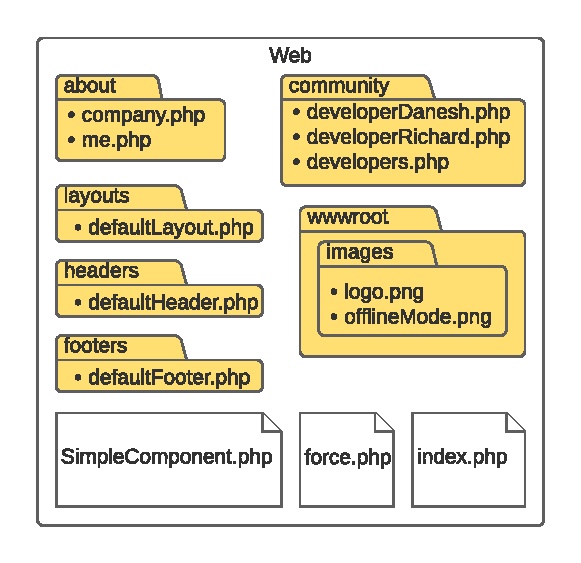
\includegraphics[scale=0.9]{./img/WebStructure}
\caption{The Web solution structure.}
\label{img22:web}
\end{figure} 
\par
An interesting page is \texttt{index.php}, which is default page of the website, shown in Figure \ref{img23:index}.
It uses script inclusion to add the head section.
Then, there is a Javascript call, which uses our predefined API, which causes showing the alert with the message when the page loads.
The whole page uses HTML interleaving.
Static resources like images can be referenced by ordinary tags.
There is also an anchor to the component defined in \texttt{SimpleComponent.php}, which can be seen in Figure \ref{img24:component}.
This page is transparently rendered by our \texttt{PhpScriptProvider}, which evaluates the whole script and adds the output as a markup text to the builder.
We can try persistent context by changing the mode.
Then, we can assign some global variable, \texttt{\$msg}, as we can see in Figure \ref{img23:index}.
When we navigate to the component, the variable remains, and we can see the content of the variable defined on the previous page.
\par
\begin{figure}[H]
\begin{lstlisting}
<?php
    require("/headers/defaultHeader.php");
    CallJsVoid("window.alert", "Hello from PHP script.");
?>
<h1>Index</h1>
...
<img src="Web/images/offlineMode.png" width="600" height="200"/>
...
Try navigating to the <a href="/simpleComponent">component</a>

<?php
    $msg="Hello from provider";
    require("/footers/defaultFooter.php");
?>
\end{lstlisting}
\caption{index.php}
\label{img23:index}
\end{figure}
\par
The \texttt{SimpleComponent} component extends our \texttt{PhpComponent} and uses \texttt{RouteAttribute} for routing.
The possibility of using attributes was added in the PHP8.0 version, and Peachpie supports them.
We can see implementing the \texttt{BuilderRenderTree} method, which uses our builder to add markup content to the page.
A more complex example of using the component we can see in \textit{PhpComponent} example.
\par
\begin{figure}
\begin{lstlisting}
<?php namespace something;
use \Microsoft\AspNetCore\Components as Microsoft;

#[Microsoft\RouteAttribute("simpleComponent")]
class ExampleComponent extends \PhpBlazor\PhpComponent {	

public function BuildRenderTree($builder) : void {
	global $msg;
	$builder->AddMarkupContent(0, "<h1>Simple component</h1>");
	$builder->AddMarkupContent(1, "<p>msg = " . $msg . "</p>");
}

}
\end{lstlisting}
\caption{SimpleComponent.php}
\label{img24:component}
\end{figure}
\par
We can see using \texttt{\$\_GET} superglobal in Figure \ref{img25:developer}, where we decide to show its content based on the URL query.
When we have the \textit{OnNavigationChanged} mode for the context, and we refresh the page after navigation to a developer, then we can see the anchors to developers.
It is caused by creating a new context between navigation, so the variables are disposed.
With the second mode, we still have the info page of the firstly navigated developer because the variables in the context remain.
\par
\begin{figure}[H]
\begin{lstlisting}
<?php
    require("/headers/defaultHeader.php");
?>
<?php
if (isset($_GET["developer"])) { 
    $name = $_GET["developer"];
    require("/community/developer$name.php");
} else {
?>
...
<p>Get more info about 
<a href="/community/developers.php?developer=Richard">Richard</a>.
</p>
...
<?php } ?>
<?php
    require("/footers/defaultFooter.php");
?>
\end{lstlisting}
\caption{developers.php}
\label{img25:developer}
\end{figure}

\section{OneScript}

In this example, we aim at the second use case.
The solution contains four project again.
\texttt{Blazor.Server} and \texttt{Peachpie.Blazor} are same.
\texttt{Blazor.Client} contains now common Razor pages, and has \texttt{Router} as a root component.
We create several scripts in the \texttt{Scripts} project to enrich the website with content generated from the PHP scripts.
The website contains three Razor pages: \texttt{Index.razor}, \texttt{PhpGateway}, and \texttt{PhpScript}.
The first page uses \texttt{PhpScriptProvider} to navigate \texttt{index.php}.
Using the provider is straightforward.
\par
We want to show the calling PHP function from Javascript in Figure \ref{img26:index}.
As we can see, it is effortless to call it.
The \texttt{callPHP} function accepts the function name and object to serialize as an function parameter.
When the script is rendered, the context contains defined \texttt{CallPHP} function.
We click on the button, which invokes \texttt{Call} method on the context, which invokes the desired function.
Then, we deserialize the parameter.
There is an interesting thing about using \texttt{echo}, \texttt{print}, etc. when the script is not rendered.
The context provides the second writer, which uses \texttt{Console} as the output.
It causes printing the message into the web browser console.
\begin{figure}
\begin{lstlisting}
...
<p>Click and look at console output</p>
<button onclick="window.php.callPHP('CallPHP',
	{ name : 'Bon', surname: 'Jovi'});">PHP</button>
<?php

function CallPHP($data)
{
    $json = json_decode($data); 

	echo "Hello " . $json->name . " ";
	echo $json->surname .  " from PHP\n";
}
\end{lstlisting}
\caption{index.php}
\label{img26:index}
\end{figure}
\par
Another part of the website uses forms to demonstrates \texttt{GET} and \texttt{POST} method.
We can see it in \texttt{php} folder, where are three examples of forms using both methods and file loading.
These examples can be navigated based on their names due to the unspecified URL of the Razor page, which uses the provider.
After navigation to this page, the provider gets the script name from the URL.
\par
\begin{figure}[!b]\centering
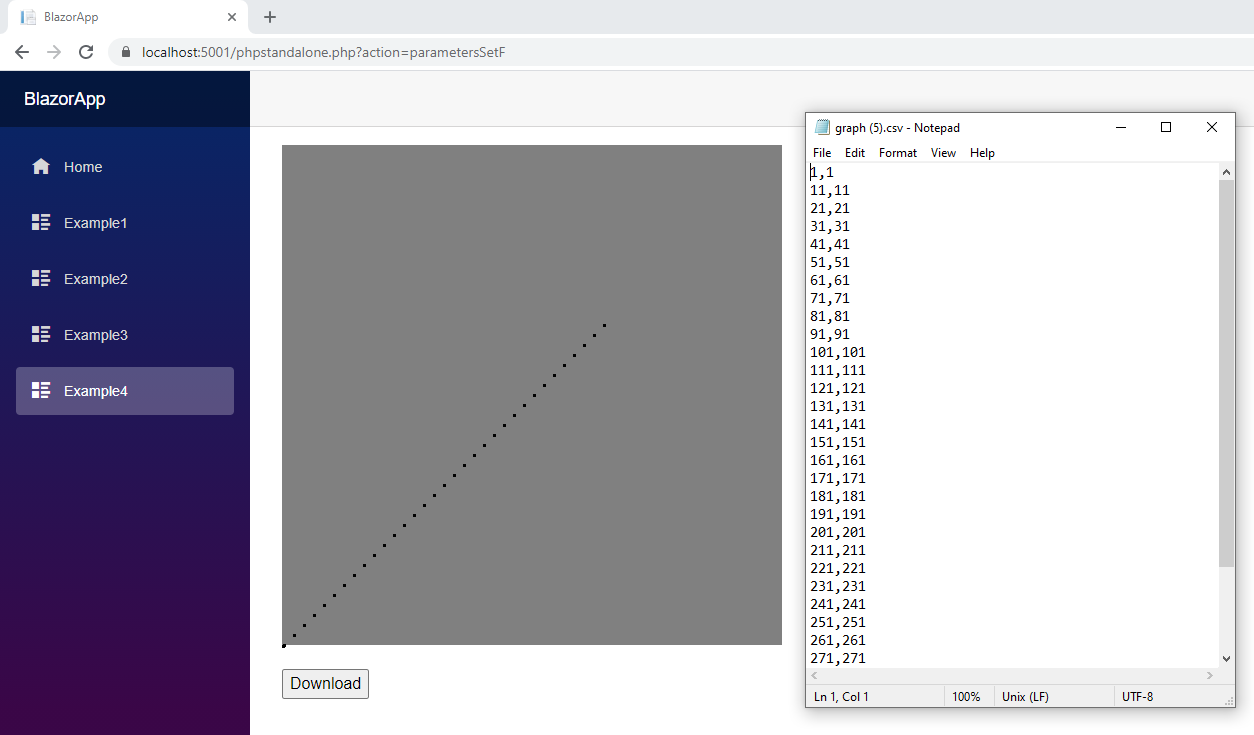
\includegraphics[scale=0.4]{./img/graph}
\caption{Application for visualising a graph.}
\label{img27:graph}
\end{figure} 
\par
The last part aims at the persistent context and using forms as interaction with the user.
It is a common approach in PHP, and we can use it on a client side due to our solution.
There is a simple application enabling us to visualize a graph, as we can see in the folder \texttt{fileManagment}.
The application can upload a CSV file containing a graph or generate a new one based on the given parameters.
It then visualizes the graph and enables it to be downloaded as a CSV file, which can be used for the next visualization, as shown in Figure \ref{img27:graph}.
We use PHP library for parsing the file, which demonstrates a possibility to utilize the already created library on a client side.
The application has the main script,\texttt{fileManagment/index.php}, which recognizes what to do based on superglobals and saved variables.
It is possible due to context persistence.

\section{PhpComponent}
\section{AllTogether}